\begin{table*}[t]
    \setlength{\belowcaptionskip}{-0.2cm}
    % \renewcommand{\arraystretch}{1.2}
    \Large
    \centering
    \resizebox{0.35\textwidth}{!}{
    \begin{tabular}{lc|cc}
        \toprule
        Source & Reference & WER$\downarrow$ & SIM$\uparrow$  \\
        \midrule
        \multicolumn{2}{c}{Groundtruth} & 0.4 & 0.93 \\
        RVQ-1 & RVQ-2 &  2.6 & 0.72 \\
        RVQ-1 & RVQ-2:4 & 11.7 & 0.80 \\
        % RVQ-1 & RVQ-2:6 & 24.2 & 0.81 \\
        RVQ-1 & RVQ-2:8 & 35.4 & 0.82 \\
        \bottomrule
    \end{tabular}}
    \caption{Results of one-shot voice conversion. Source and Reference refers to source token matrix and reference token matrix respectively. 
    }
    \label{tab:oneshot_vc}
\vspace{-1em} 
\end{table*}

\begin{figure*}[t] 
    % \setlength{\abovecaptionskip}{-0.cm}
    % \setlength{\belowcaptionskip}{-0.5cm}
    \centering 
    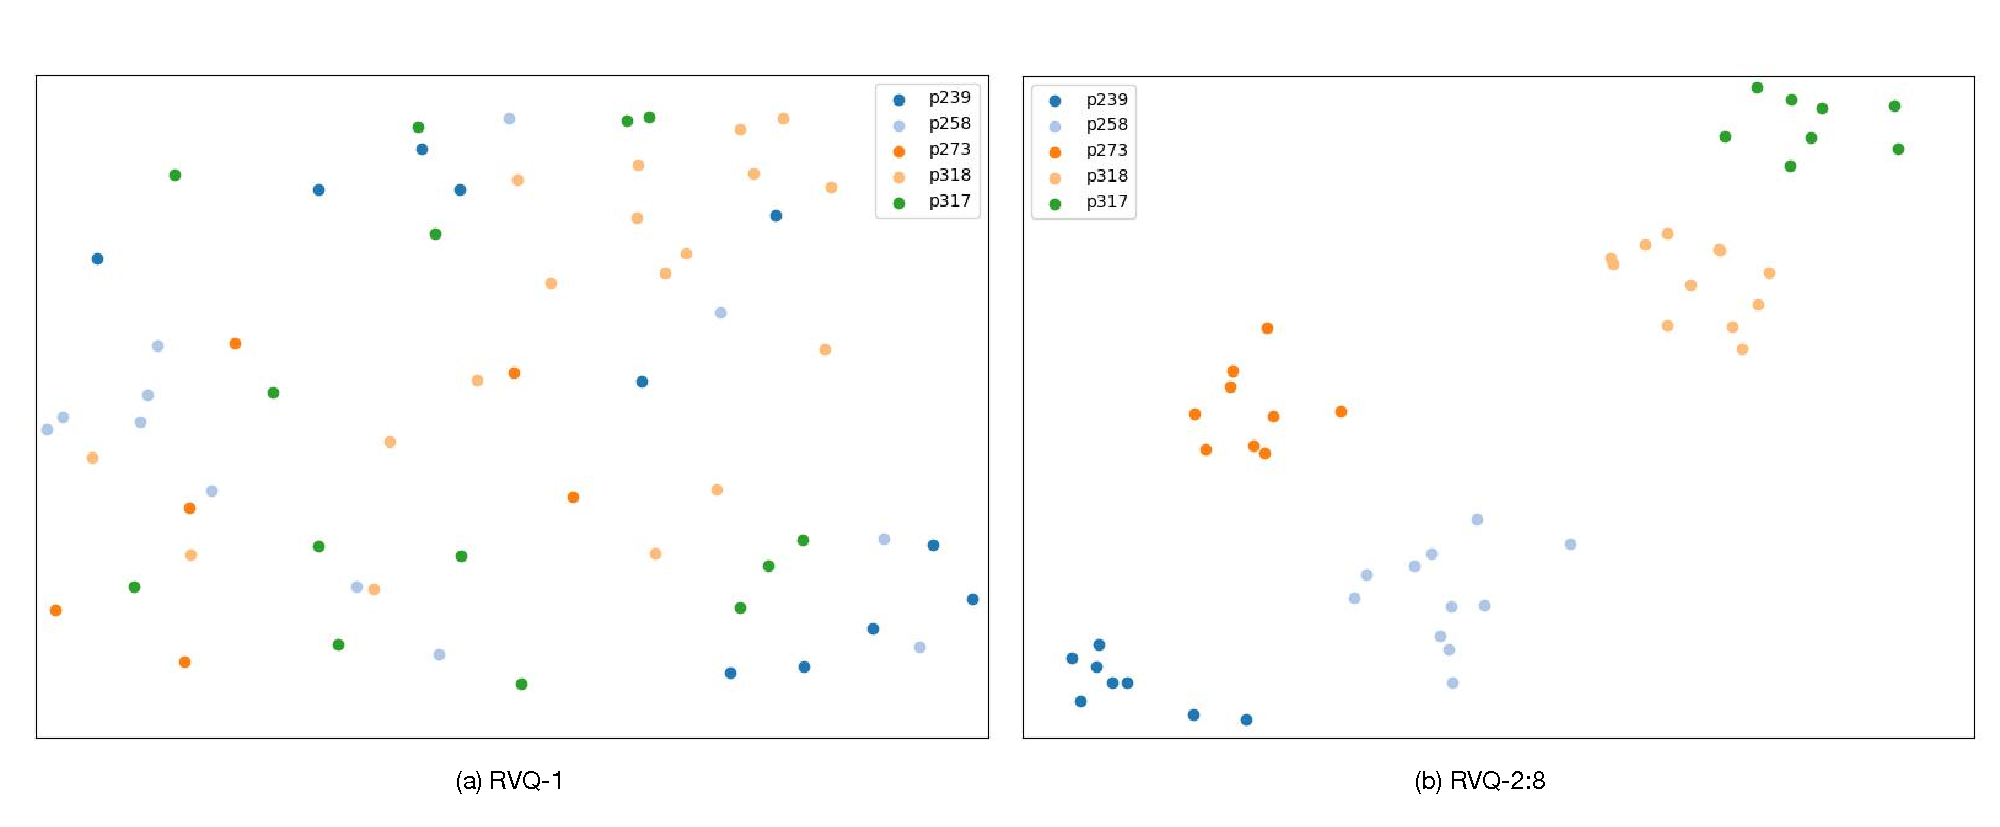
\includegraphics[width=0.8\textwidth]{Figures/spk_emb.pdf} 
    \caption{Visualization of quantized output of different RVQ layers of \method.The first layer is denoted as RVQ-1, while the sum of the second layer to the eighth layer is denoted
    as RVQ-2:8.}
    \label{fig:spk_emb} 
\vspace{-1.5em} 
\end{figure*}

To demonstrate that different speech information can be hierarchically modeled in \method, we conduct one-shot voice conversion~(VC) experiment. This experiment aims to convert speech from any source speaker to an arbitrary target speaker using only a few seconds of reference speech from the target speaker. 
To use \method for one-shot VC, the first step is to transform the source speech and reference speech into token matrices. 
By concatenating the RVQ-1 tokens of source token matrix with RVQ-2:8 tokens of the reference token matrix, and then passing this combined token matrix to the decoder, we can achieve voice conversion. 
The lengths of the reference and source tokens may not align perfectly. To address this, we use truncation or circular padding to ensure they share the same temporal length, thereby facilitating the concatenation process.
We conduct experiments on VCTK dataset. We randomly selected one speech sample from a speaker to serve as the source speech. From the remaining 107 speakers, we individually selected one speech sample of different content to act as the reference speech. We employed two metrics for evaluation: WER and speaker similarity.

Table~\ref{tab:oneshot_vc} reports the results of one-shot VC experiments. From the table, we can see that as the number of layers for reference tokens increases, speaker similarity also gradually increases. This suggests that more information from the reference speaker is being transferred over, proving that speaker information is embedded in tokens from the second to the last layers. When the reference tokens are selected from the second to the fourth layers, we achieve low WER and high speaker similarity, resulting in a satisfactory one-shot VC performance. This indicates that the information disentanglement is successful. 
% We put samples of one-shot VC on our demo page~\footnote{\url{https://0nutation.github.io/SpeechTokenizer.github.io/}}.

We also visualize quantized outputs from different layers in Figure~\ref{fig:spk_emb}. 
Specifically, We randomly select five speakers from the VCTK dataset and pick 10 random speech samples per speaker. We extract quantized output of different RVQ layers of \method. The first layer output is denoted as RVQ-1 representations, while the sum of the outputs from the second layer to the eighth layer is denoted as RVQ-2:8 representations. By performing mean pooling along the temporal dimension, each representation is converted into a single vector. These vectors are then visualized in a 2D space using t-SNE, with speech samples from the same speaker represented in the same color.
From the plot, it can be observed that the RVQ-1 representations for different speakers are scattered randomly without discernible pattern. In contrast, the RVQ-2:8 representations for the same speaker tend to cluster together, while being distinct from those of other speakers. This suggests that speaker-specific information is contained from the second layer up to the eighth layer.

% 从VCTK中随机选择5个说话人并且每人随机选10条语音，我们用\method提取离散code并在对应codebook中找到对应的连续vector。通过在时间维度上做mean pooling，每条语音变成一个向量。我们可视化它们in 2D space with t-SNE in Figure~\ref{fig:spk_emb}. 相同说话人的语音用同一个颜色表示。从图中可以看到不同说话人的RVQ-1的表示分布混在一起，没有规律。而同一个说话人的RVQ2:8的表示聚在一起，说明说话人信息蕴藏在the second layer to the eighth layer.

% 从表中我们可以看到，随着reference token的层数的增加，speaker similarity在逐渐增加，说明越多的reference speaker的说话人信息被迁移过来，说话人信息蕴藏在第二层到第八层的token中。当reference token选择二到四层时，取得了不错的WER和speaker similarity，获得不错的one-shot VC的效果，说明信息解耦是成功的。

% 为了证明\method中实现了有效的信息解耦，不同的语音信息能够在speech token中分层建模，我们进行了one-shot voice conversion~(VC)的实验，which aims to convert speech from any source speaker to an arbitrary target speaker with only a few seconds of reference speech from the target speaker。使用\method来进行one-shot VC的具体做法为首先把source speech和reference speech变成token matrix，将source token matrix的第一层token，和reference token matrix的后面几层token拼接后送到decoder中获得语音，来实现voice conversion.
% 我们在VCTK数据集上做了实验，随机选择一个speakr的一条语音作为source speech，在其他107个speaker中各随机选择一条具有不同内容的语音作为reference speech。我们使用WER和speaker similarity来evaluateone-shot VC的performance。


